% !TEX TS-program = xelatex
% !TEX encoding = UTF-8 Unicode
% WORKING!!!! File encoding: UTF-8 - file need be saved as utf8
%             Latex encoding:UTF-8 - need package utf8

\documentclass[12pt]{article}
% Margins
\usepackage[a4paper]{geometry}
\geometry{verbose,tmargin=2.5cm,bmargin=2cm,lmargin=2cm,rmargin=2cm}

%==============================================================================
% Imports
%==============================================================================
% UTF-8
\usepackage[utf8]{inputenc}
% Math formulas
\usepackage{amsmath}
% Graphics
% \usepackage{graphicx} 
% Page view
\usepackage{fancyhdr}
% Matlab codes
% To use this library add mcode.sty to same folder.
% \usepackage[]{mcode}
% Subfigure caption
\usepackage{subcaption}
% Line spacing
\usepackage{setspace}
% Specific symbols (degree...)
\usepackage{gensymb}
% For function description
\usepackage{cmap}
\usepackage[T1]{fontenc}
\usepackage{times}
\usepackage[Bjarne]{fncychap}
\usepackage{longtable}
\usepackage{sphinx}
\usepackage{multirow}

%==============================================================================
% Settings
%==============================================================================
%\renewcommand{\thesection}{ \arabic{section}}
\pagestyle{fancy}
\fancyhf{}
\usepackage{titling}
\fancyhf[HC]{\thetitle}
\fancyhf[HL,HRO]{\theauthor}
\fancyhf[HR,HLO]{\today}
\fancyhf[FL,FRO]{\thepage}
% Paragraph spacing
\setlength{\parindent}{0em}
% Line spacing
\onehalfspacing

%==============================================================================
\title{Program for measurement and calibrating data from observatory
    variometer}
\author{Albershteyn Andrey \\ 
    \href{mailto:alberand@fel.cvut.cz}{alberand@fel.cvut.cz}}

\date{\today}

\begin{document}

\maketitle

%==============================================================================
% 1
%==============================================================================
\renewcommand*\contentsname{Contents}
\tableofcontents
%==============================================================================
% 2
%==============================================================================
\section{Description}
\par This program is used for data calibration and saving it. Data is received
from observatory variometer by the serial bus. Main purpose of this software is 
to be easy to use and correctly working on Raspberry Pi.
\par Sensor contains FPGA chip which create data stream and send it via serial
port. Sensor is connected to voltage level converter and than to the Raspberry
Pi's serial interface.
\par Program is separeted into 3 different processes. First 'main' process is 
main flow of program. It communicates with sensor and receivs raw data from it.
Second process 'processor' is responsible for data calibration, third process
just saves calibrated data to files. Processes are connected by two pipelines 
and they are independent, only in case of terminating main process 'main', other
processes will be terminated.
\newline
\par This program have a few test function, for debugging. One of them is that
program will indicate every received sample by changing state of one of GPIO
pins. This pin can be choosen in configuration file, by default it's pin 4. Its
can be used for confirming that all samples sent by serial port are received by
Raspeberry Pi.
\par Other option is that we can run program in virtual mode and we don't need
real sensor for it. In this mode program generate random data and use it as a
input stream. It can be used for verification that calibration is working right
way. And test program's functionality.
\par Also you can turn on logging for whole program cycle. Program contains
information messages in different places to inform user about current performed
task. This option is possible to turn on/off in configuration file.
\newline
\par Whole program is write with using only built-in python libraries. So it
don't need third-party software. Only if debug mode is turned on (thus some of
the GPIO pin is used for samples indication) it is necessary to install GPIO
library to communicate with pins. Program is written in Python 3.2, so it should
be compatible with all Python 3.* versions.
%==============================================================================
% 3
%==============================================================================
\section{Program's structure}
\par In this section we have program's structure. That is  what is every file
responsible for and how it connected.
\begin{figure}[htb!]
    \centering
    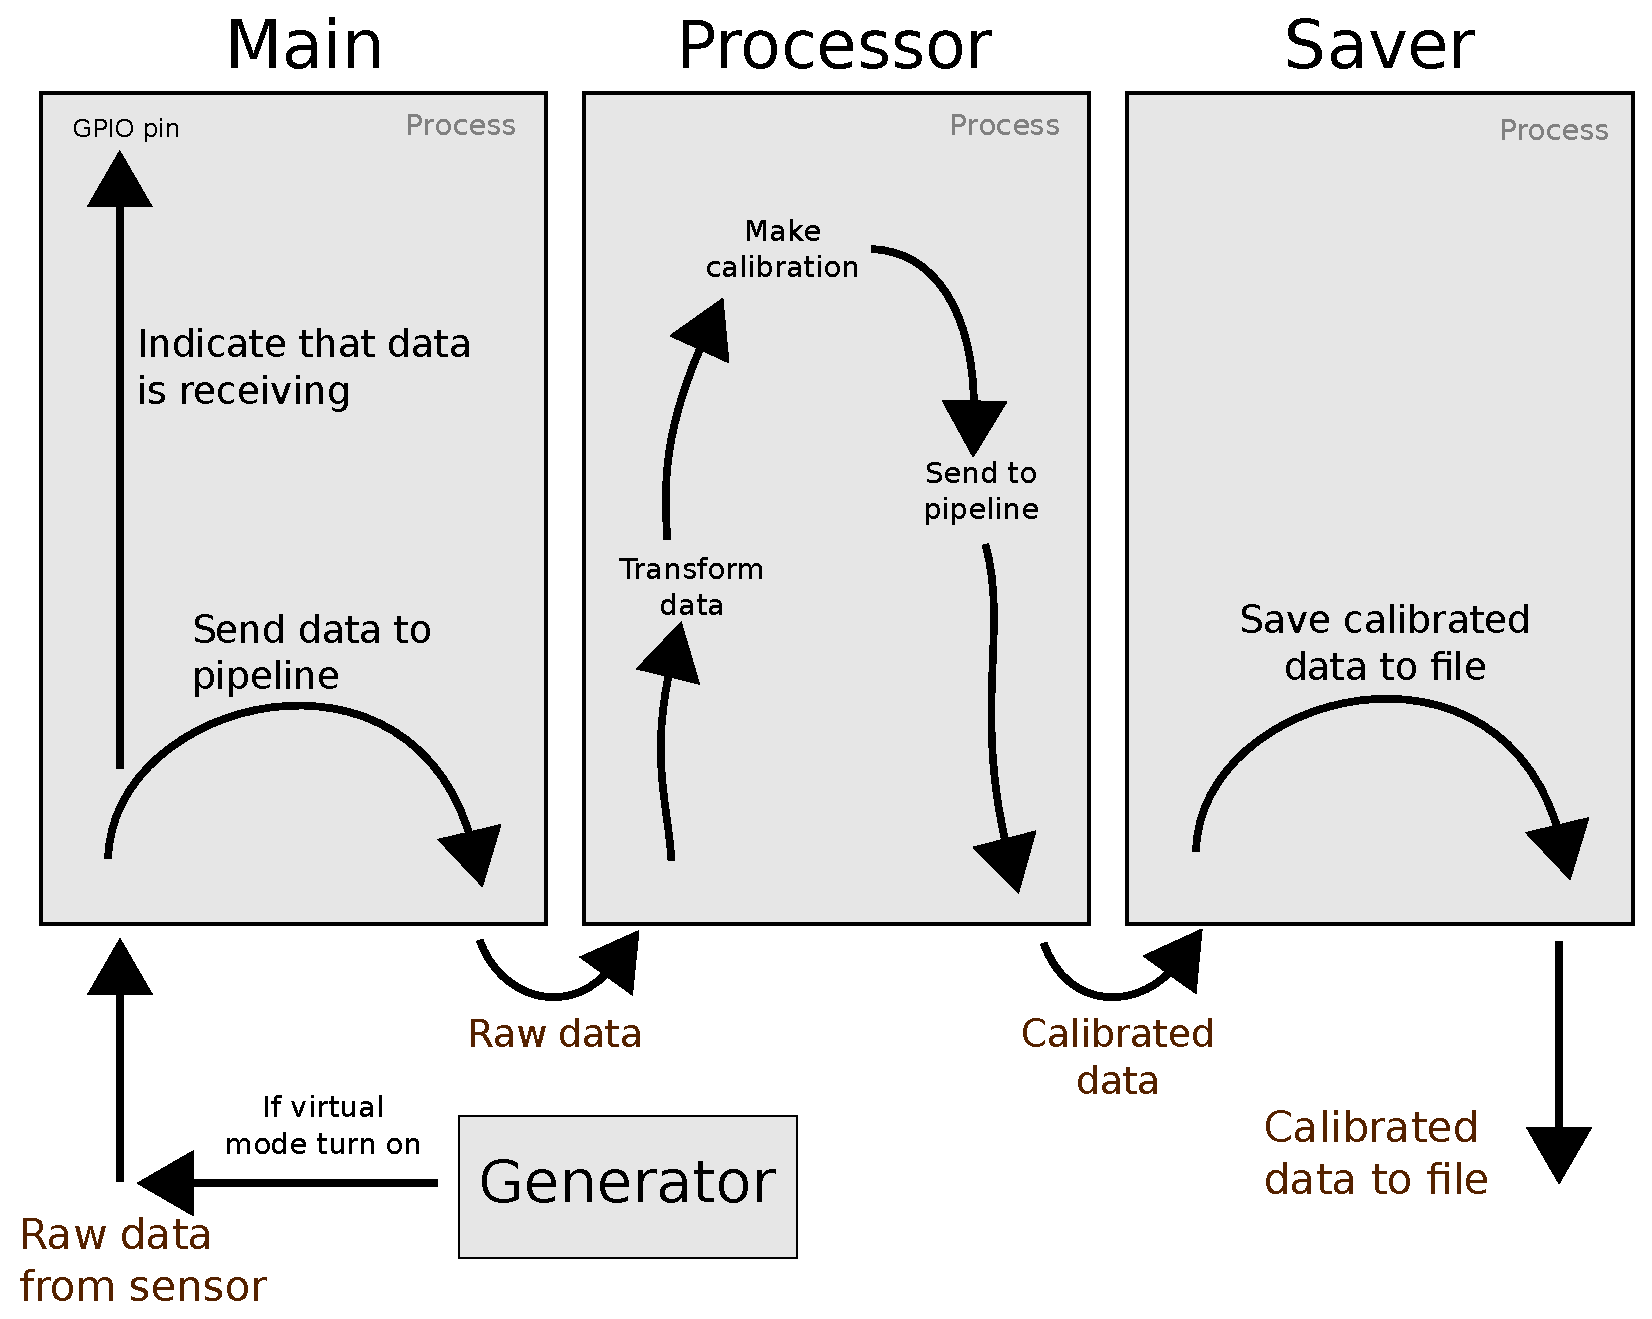
\includegraphics[width=0.7\textwidth]{./structure_v3.eps}
\end{figure}

\par Files' list:
\begin{enumerate}
    \item \textbf{main.py} - This file is main input point to the program.
        Runs as a separated process and perform data reading from serial port 
        and than send it to pipeline to following calibration. 
    \item \textbf{saver.py} - contains only one function, which is run as a
        separated process and perforn data saving. 
    \item \textbf{calibration.py} - contains a few utility function, which are
        used in processor for data calibration and some data transformation. 
    \item \textbf{processor.py} - contains one function, which is run as a
        separate process. Perform data calibration and send calculated value to
        pipeline to saving process.
    \item \textbf{reader.py} - this file contains functions for serial
        communication setup and functions for communication with device. 
    \item \textbf{generator.py} - contains class, which is used as a generator
        of random numbers. It's used only in debug mode, when we don't have real
        sensor we use this generator to test program functionality.
    \item \textbf{settings.py} - this file contains two classes which are
        responsible for program and calibration settings (next section).
\end{enumerate}


%==============================================================================
% 4
%==============================================================================
\section{Configuration settings}
\par In this section we have description of configuration file. Program have two
configuration classes. One for program configuration (where to store data files,
turn on/off debug mode, serial communication settings etc.), second class is
responsible for data calibration (offsets, sensitivitiy etc.)
\par Program configuration:
\begin{enumerate}
    \item \textbf{samples} - number of sampels received per second.
    \item \textbf{debug} - Turn on or turn off debug mode. Thus, program will
        indicate every sample on debug pin by sending impuls and all program's
        action will be logged.
    \item \textbf{debug\_pin} - GPIO pin which is used to indicate samples
        receving. Thus, this pin will change his state before and after data
        sample.
    \item \textbf{path} - path where program will be store all files.
    \item \textbf{port} - port for serial communication. Sensor should be
        connected to this port. By default port is '/dev/ttyAMA0'.
    \item \textbf{baudrate} - serial communication speed. By default, speed is
        set up to 115 200.
    \item \textbf{timeout} - timeout for serial communication. By default, value
        is 3.
    \item \textbf{start\_cmd} - string command, which is send to sensor to start
        it. Starts data stream.
    \item \textbf{stop\_cmd} - string, which is send to the sensor to stop it.
    \item \textbf{file\_name\_format} - string, which define how filename will
        looks like.
\end{enumerate}
\par Calibration settings:
\begin{enumerate}
    \item \textbf{comp} - the compensation field
    \item \textbf{ofs} - offsets
    \item \textbf{sen} - sensitivity
    \item \textbf{ort\_mat} - the orthogonalization matrix
\end{enumerate}
%==============================================================================
% 5
%==============================================================================
\section{Functions' documentation}
\par Description of functions
\begin{fulllineitems}
\phantomsection\label{index:calibration.calibrate}\pysiglinewithargsret{\code{calibration.}\bfcode{calibrate}}{\emph{data}}{}
This function calibrate data and return numpy array. (np is numpy)
\begin{quote}\begin{description}
\item[{Parameters}] \leavevmode
\textbf{\texttt{data}} -- is list with 3 items. For example: np.array({[}123, 456, 789{]})

\item[{Returns}] \leavevmode
np.array({[}111, 444, 777{]}) array with calibrated data

\end{description}\end{quote}

\end{fulllineitems}

\index{find\_mean() (in module calibration)}

\begin{fulllineitems}
\phantomsection\label{index:calibration.find_mean}\pysiglinewithargsret{\code{calibration.}\bfcode{find\_mean}}{\emph{data}, \emph{gauss}}{}
This function apply gauss filter to data and then calculate mean value. And
multiply it by 2.
\begin{quote}\begin{description}
\item[{Parameters}] \leavevmode
\textbf{\texttt{data}} -- np.array({[}{[}H{]}, {[}Z{]}, {[}E{]}, {[}T{]}{]}). H, Z, E and T are arrays

\item[{Returns}] \leavevmode
np.array({[}{[}H{]}, {[}Z{]}, {[}E{]}, {[}T{]}{]})

\end{description}\end{quote}

\end{fulllineitems}

\index{parse\_data\_string() (in module calibration)}

\begin{fulllineitems}
\phantomsection\label{index:calibration.parse_data_string}\pysiglinewithargsret{\code{calibration.}\bfcode{parse\_data\_string}}{\emph{string}}{}
Cut string from sensors to separate values.
\begin{quote}\begin{description}
\item[{Parameters}] \leavevmode
\textbf{\texttt{string}} -- string in format like this `1234567123456712345671234567'

\item[{Returns}] \leavevmode
{[}1234567, 1234567, 1234567, 1234567{]}

\end{description}\end{quote}

\end{fulllineitems}

\index{save\_data() (in module calibration)}

\begin{fulllineitems}
\phantomsection\label{index:calibration.save_data}\pysiglinewithargsret{\code{calibration.}\bfcode{save\_data}}{\emph{data}, \emph{path}, \emph{suffix='`}}{}
Save data to path/\%Y-\%m-\%d\_suffix.txt
\begin{quote}\begin{description}
\item[{Parameters}] \leavevmode\begin{itemize}
\item {} 
\textbf{\texttt{data}} -- some data (For example: 123 123 123)

\item {} 
\textbf{\texttt{path}} -- path where to save file (For example: ./data/)

\item {} 
\textbf{\texttt{suffix}} -- suffix for filename (For example for suffix `original' filename
will be 2015-12-24\_original.txt)

\end{itemize}

\end{description}\end{quote}

\end{fulllineitems}

\phantomsection\label{index:module-generator}\index{generator (module)}\index{Generator (class in generator)}

\begin{fulllineitems}
\phantomsection\label{index:generator.Generator}\pysigline{\strong{class }\code{generator.}\bfcode{Generator}}
Bases: \code{object}

This class is used only in `Virtual' mode. In this mode we are don't have
connected sensor and just generate random values for test program. So this
class implements basic function of serial port.
\index{read() (generator.Generator method)}

\begin{fulllineitems}
\phantomsection\label{index:generator.Generator.read}\pysiglinewithargsret{\bfcode{read}}{\emph{number\_of\_byte}}{}
This function return string in this format:
1234567;1234567;1234567;1234567;
Numbers are just random.
\begin{quote}\begin{description}
\item[{Parameters}] \leavevmode
\textbf{\texttt{number\_of\_byte}} -- not used

\item[{Returns}] \leavevmode
string

\end{description}\end{quote}

\end{fulllineitems}

\index{readline() (generator.Generator method)}

\begin{fulllineitems}
\phantomsection\label{index:generator.Generator.readline}\pysiglinewithargsret{\bfcode{readline}}{}{}
This function return string in this format:
1234567;1234567;1234567;1234567;
Numbers are just random.
\begin{quote}\begin{description}
\item[{Returns}] \leavevmode
string

\end{description}\end{quote}

\end{fulllineitems}

\index{write() (generator.Generator method)}

\begin{fulllineitems}
\phantomsection\label{index:generator.Generator.write}\pysiglinewithargsret{\bfcode{write}}{\emph{data}}{}
Just print received data.
\begin{quote}\begin{description}
\item[{Parameters}] \leavevmode
\textbf{\texttt{data}} -- string

\end{description}\end{quote}

\end{fulllineitems}


\end{fulllineitems}

\phantomsection\label{index:module-processor}\index{processor (module)}\index{process\_data() (in module processor)}

\begin{fulllineitems}
\phantomsection\label{index:processor.process_data}\pysiglinewithargsret{\code{processor.}\bfcode{process\_data}}{\emph{pipeline}, \emph{samples}, \emph{path='./'}}{}
Process data from sensor. Accordingly get n samples and calculate average
value from these samples. Then use Gauss filter and finally make
calibration.
\begin{quote}\begin{description}
\item[{Parameters}] \leavevmode\begin{itemize}
\item {} 
\textbf{\texttt{pipeline}} -- pipeline where from this function will receive samples

\item {} 
\textbf{\texttt{samples}} -- number of samples per second

\item {} 
\textbf{\texttt{path}} -- path where we will save our files

\end{itemize}

\end{description}\end{quote}

\end{fulllineitems}

\phantomsection\label{index:module-reader}\index{reader (module)}\index{init\_communication() (in module reader)}

\begin{fulllineitems}
\phantomsection\label{index:reader.init_communication}\pysiglinewithargsret{\code{reader.}\bfcode{init\_communication}}{\emph{port='/dev/ttyAMA0'}, \emph{baudrate=115200}, \emph{timeout=None}}{}
This function create Serail communication object with default parameters:
\begin{quote}\begin{description}
\item[{Parameters}] \leavevmode\begin{itemize}
\item {} 
\textbf{\texttt{port}} -- serial port. By default `/dev/ttyAMA0'

\item {} 
\textbf{\texttt{baudrate}} -- By default 115200

\item {} 
\textbf{\texttt{timeout}} -- By default `None'

\end{itemize}

\item[{Returns}] \leavevmode
pyserial object to communicate with device

\end{description}\end{quote}

\end{fulllineitems}

\index{readline() (in module reader)}

\begin{fulllineitems}
\phantomsection\label{index:reader.readline}\pysiglinewithargsret{\code{reader.}\bfcode{readline}}{\emph{inpoint}}{}
Read one line from sensor.
\begin{quote}\begin{description}
\item[{Parameters}] \leavevmode
\textbf{\texttt{inpoint}} -- pyserial object

\item[{Returns}] \leavevmode
line or False

\end{description}\end{quote}

\end{fulllineitems}

\index{start\_sensor() (in module reader)}

\begin{fulllineitems}
\phantomsection\label{index:reader.start_sensor}\pysiglinewithargsret{\code{reader.}\bfcode{start\_sensor}}{\emph{inpoint}}{}
This function send start command to sensor (`CN').
\begin{quote}\begin{description}
\item[{Parameters}] \leavevmode
\textbf{\texttt{inpoint}} -- pyserial object

\item[{Returns}] \leavevmode
True if start is successful otherwise False.

\end{description}\end{quote}

\end{fulllineitems}

\index{stop\_sensor() (in module reader)}

\begin{fulllineitems}
\phantomsection\label{index:reader.stop_sensor}\pysiglinewithargsret{\code{reader.}\bfcode{stop\_sensor}}{\emph{inpoint}}{}
Send stop command to sensor (`CS'). And return true if writing
is successful.
\begin{quote}\begin{description}
\item[{Parameters}] \leavevmode
\textbf{\texttt{inpoint}} -- pyserial object

\item[{Returns}] \leavevmode
True if stop is successful otherwise False.

\end{description}\end{quote}

\end{fulllineitems}

\phantomsection\label{index:module-saver}\index{saver (module)}\index{data\_saver() (in module saver)}

\begin{fulllineitems}
\phantomsection\label{index:saver.data_saver}\pysiglinewithargsret{\code{saver.}\bfcode{data\_saver}}{\emph{pipeline}, \emph{path='./'}}{}
This function is run as a process and its save data getted from pipeline.
\begin{quote}\begin{description}
\item[{Parameters}] \leavevmode\begin{itemize}
\item {} 
\textbf{\texttt{pipeline}} -- pipeline

\item {} 
\textbf{\texttt{path}} -- path where to save data

\end{itemize}

\end{description}\end{quote}

\end{fulllineitems}

\end{document}
